\chapter{}
\section{确定一个物质的Lewis结构式}
\label{sec:1.1}
确定一个物质的lewis结构式$\rightarrow$机理:载体

物质
$\begin{cases}
    \text{中性分子} \\
    \text{自由基(中性):特殊自由基Cl氯自由基} \\
    \text{离子(带电)}
\end{cases}$

形成过程中发生了$e^-$的转移/迁移

\subsection{简单分子}
\label{sec:1.1.1}
依据:简单原子核外的电子排布+Lewis$\uwave{\text{电子配对}}$学说

氧$\underset{\text{原子实}}{\underline{{+8\quad 2}}}\underset{\text{+价层电子}}{\underline{6}}$=原子核+核外电子

$\uwave{\text{八隅体规则}}$:
尽量配出$8e^-$稳定结构(II周期)

$\chemfig{O(-[:-140]H)(-[:-40]H)}\rightarrow
\begin{cases}
    \text{O原子独享}
    \begin{cases}
        \text{孤电子} \\
        \text{未共享$e^-$}
    \end{cases} \\
    \text{$4e^-$位于O-H:成键电子}
\end{cases}$

\subsection{简单自由基}
\label{sec:1.1.2}
$\begin{cases}
    \underset{\text{(使满足八隅体规则的原子尽可能多)}}{\text{配对法$\rightarrow$两个电子配对成化学键}}\\
    \text{结构未知推导法:均裂思想}
\end{cases}$

$\overset{2e^-}{\overset{\uparrow}{\ce{CH_3-H}}}\ce{->}\underset{\text{均裂:中性分子$\rightarrow$中性自由基}}{\underset{\downarrow}{\ce{*CH_3 + H*}}}$

\subsection{简单离子}
\label{sec:1.1.3}
离子形成一定有电子的转移
$\begin{cases}
    \text{中性物质得}e^-\rightarrow\text{阴离子}^{\ominus} \\
    \quad \downarrow \\
    \text{自由基} \\
    \quad \uparrow \\
    \text{中性物质失}e^-\rightarrow\text{阳离子}^{\oplus}
\end{cases}$

$\ce{*CH_3 -> ^{\oplus}CH_3 + e^-}$

$\ce{e^- + *CH_3 -> ^{\ominus}CH_3}$

异裂思想: $\ce{A-B ->[\text{异裂}]}\underset{\text{相反电性}}{\ce{A^{\oplus} + B^{\ominus}}}$

$\chemfig{
    C(-[:0]H)
    (-[:180]C([:0])(-[:180]H)(-[:-90]H)(-[:90]H))
    (-[:-90]H)(-[:90]H)}
    \ce{->}
    \underset{\text{1孤对电子}}{\underset{\text{3对成键电子}}
    {^{\ominus}\chemfig{C(-[:0]H)([:180])(-[:-90]H)(-[:90]H)}}}
    +
    \underset{\text{无孤对电子}}{\underset{\text{3对成键电子}}
    {^{\oplus}\chemfig{C(-[:0]H)([:180])(-[:-90]H)(-[:90]H)}}}$

\subsection{标记形式电荷}
\label{sec:1.1.4}

\chemfig{C^{\oplus}(-[:0])(-[:180])([:-90])(-[:90])}
\qquad
\chemfig{C^{*}(-[:0])(-[:180])([:-90])(-[:90])}
\qquad
\chemfig{C^{\ominus}(-[:0])(-[:180])([:-90])(-[:90])}

形式电荷(与真实电荷有区别),某些情况真的只是“形式电荷”

公式:
形式电荷=主族序数-不包括单电子的未共享电子数
$\underset{\textcolor{red}{\text{也会把单电子看作化学键}}}{\underset{\textcolor{red}{\text{化学键数}}}{\underline{\text{$-\frac{1}{2}$成键电子数}}}}$

$\underset{4-2-4=0}{\chemfig{C(-[:0])(-[:180])([:-90])(-[:90])}}
\begin{matrix}
    \ce{->[\text{得$e^-$}]}\chemfig{C^{\ominus}(-[:0])(-[:180])([:-90])(-[:90])}:4-2-3=-1 \\
    \ce{->[\text{失$e^-$}]}\chemfig{C^{\oplus}(-[:0])(-[:180])([:-90])(-[:90])}:4-0-3=+1
\end{matrix}$

$\chemfig{O^{\oplus}(-[:0])(-[:180])(-[:90])}\quad 6-2-3=+1$

\qquad $\downarrow$

\quad $\ce{H_3O^{\oplus}}\Rightarrow\chemfig{O(-[:90]H)(-[:-150]H)(-[:-30]H)}(sp^3)\rightarrow$对于
$\underset{\chemfig{O^{\oplus}(-[:90]H)(-[:-150]H)(-[:-30]H)}\checkmark}{\ce{H_3O^+,}}$是不标O上的孤对电子

\subsection{“复杂”分子的Lewis结构式}
\label{sec:1.1.5}
CO:
$\ce{C-O -> C=O ->}\overset{\text{C不满足八隅体规则}}{\ce{O^{\oplus} ->[==] C^{\ominus}}}$
配位键:$\underset{\text{$\delta+/\delta-$部分电荷中心}}{\overset{\delta-}{\ce{C}}\ce{<-[==]}\overset{\delta+}{\ce{O}}}$

NO(长命自由基):
$\overset{7e^-}{N}=\underset{8e^-}{O}\quad 6-4-2=0$

\subsection{总结}
\label{sec:1.1.6}
书写Lewis结构$\rightarrow$配对电子+标志形式电荷

1.公式法
$\begin{cases}
    \text{原子序数} \\
    \text{化学键数} \\
    \text{未共享电子数}
\end{cases}$
2.灵活性
$\begin{cases}
    \text{知道自由基}
    \begin{cases}
        \text{得$e^-$} \\
        \text{失$e^-$}
    \end{cases} \\
    \underset{\text{大多数机理}}{\text{中性分子}}
    \begin{cases}
        \underset{\text{(化学键)}}{\text{异裂思想}} \\
        \text{配位键}
        \begin{cases}
            \text{进攻:形式电荷+1} \\
            \text{被进攻:形式电荷-1}
        \end{cases}
    \end{cases}
\end{cases}$

$\qquad\qquad\underset{\text{进攻者}}{\overset{0\rightarrow+1}{\oplus}O}
\overset{\textcolor{red}{\rightarrow}}{=}
\underset{\text{被进攻者}}{\overset{0\rightarrow-1}{C:\ominus}}$

形式电荷$\&$部分电荷中心

形式电荷$\oplus/\ominus
\begin{cases}
    \text{在简单离子中表示带电情况} \\
    \text{在复杂体系中不能理解为电性分布} \\
    \text{但是能提现Lewis结构式中的价电子数}
\end{cases}$

部分电荷中性$\delta+/\delta-
\begin{cases}
    \text{物理意义:表示每个原子实的电性(静电势)} \\
    \text{在简单体系中可以使用电负性来预测} \\
    \text{如今常使用计算软件表征分子的静电势}
\end{cases}$

\section{原子轨道,价层$e^-$,杂化轨道}
\label{sec:1.2}
原子轨道简述,价层电子互斥理论,杂化轨道理论

以$H_2O$的Lewis结构式为例
$\chemfig{O(-[:-140]H)(-[:-40]H)}
\begin{cases}
    \underset{\text{成键的本质?}\rightarrow Lewis \rightarrow VBT \rightarrow MO}{\text{优点:知道较为确切成键情况}} \\
    \text{缺点:}\underset{\text{杂化VSEPR}}{\underset{\downarrow}{\underset{\text{分子的$\underline{\text{空间结构}}$?}}{\text{运动范围未知}}}}
    \rightarrow
    \underset{\text{轨道}}{\underline{\text{单原子$\rightarrow$多原子分子}}}
\end{cases}$

\subsection{什么是轨道(orbital)}
\label{sec:1.2.1}
什么是$\overset{\text{原子轨道理论(AOT)}}{\overset{\uparrow}{\text{轨道(orbital)}}}$

\qquad\qquad Bohr:电子围绕原子核的稳定$\overset{\textcolor{red}{\text{形象}}}{\underline{\text{轨道}}}$上运动

现代意义\quad $\text{解Schrödinger方程}\rightarrow\text{轨道}\rightarrow$分布

$H=\underset{\text{动能}}{T}+\underset{\text{势能}}{V}
\hfill
H\ket{\Psi}=E\ket{\Psi}
\hfill
\Psi:\text{波函数}\rightarrow\text{描述电子的“运动”}$

\begin{figure}[H]
    \begin{tikzpicture}[baseline=(current bounding box.center),scale=.5]
        \draw[-](1,3.5)--++(1,0)node[right]{能量大};
        \draw[-](1,3)--++(1,0);
        \draw[-](1,2.5)--++(1,0);
        \draw[-](1,2)--++(1,0);
        \draw[-](1,1.5)--++(1,0);
        \draw[-](1,1)--++(1,0);
        \draw[-](1,0.5)--++(1,0);
        \draw[-](1,0)--++(1,0)node[right]{能量小};
        \node[right] at (0.8,-1){能级};
        \draw[->](0,0)--(0,4)node[right]{Eorb};
    \end{tikzpicture}
    $\begin{cases}
        \text{轨道的分布$\rightarrow$几何关系} \\
        \text{轨道的能力$\rightarrow$大小关系}
    \end{cases}$
    \hfill
    \begin{subcaptionbox}
        \begin{tikzpicture}[baseline=(current bounding box.center),scale=.5]
            \coordinate (center) at (0,0);
            \foreach \r in {1, 2} {\draw (center) circle (\r cm);}
            \draw[red] (center) circle (1.5);
            \draw[->](1.5,0)--(2.5,-0.8)node[right]{节面};
            \node[right] at (2,1) {2s};
            \node[right] at (0,0) {1s};
          \end{tikzpicture}
    \end{subcaptionbox}
\end{figure}

\subsubsection{1.2.1.1轨道的分布}

在笛卡尔坐标系的$\underset{\text{不同的区域}}{\underline{\text{几何表示}}}
\left.\begin{matrix} 
    \left\{\begin{matrix} 
    \text{形态不同} \\  
    \underset{\textcolor{red}{\text{(颜色)}}}{\text{符号不同}} 
    \end{matrix}\right. 
\end{matrix}\right\}\underset{\text{(相位)}}{\text{是否拥有节面}}$

\begin{figure}[H]
    \begin{tikzpicture}[baseline=(current bounding box.center),scale=.7]
        \draw[-](0,0.5)--node[above,pos=0.5]{正相位}(3,0.5)node[right]{$\Psi>0$};
        \draw[->](0,0)--(3,0)node[right]{x};
    \end{tikzpicture}
\end{figure}
  
\begin{figure}[H]
    \centering
    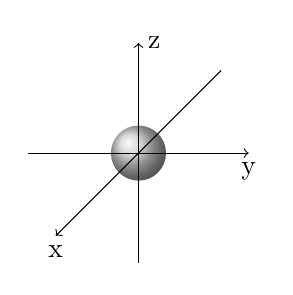
\begin{tikzpicture}[baseline=(current bounding box.center),scale=.7]
        \shade[ball color=black!20] (0,0)circle (0.5);
        \draw[->](-2,0)--(2,0)node[below]{y};
        \draw[->](1.5,1.5)--(-1.5,-1.5)node[below]{x};
        \draw[->](0,-2)--(0,2)node[right]{z};
    \end{tikzpicture}
    \caption{s轨道的几何分布}
    \label{f1.1}
\end{figure}

\begin{figure}[H]
    \centering
    \begin{subcaptionbox}
        \centering
        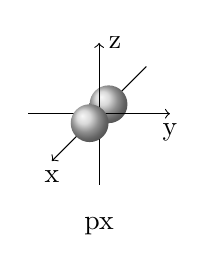
\begin{tikzpicture}[baseline=(current bounding box.center),scale=.6]
            \draw[->](1,1)--(-1,-1)node[below]{x};
            \shade[ball color=black!20] (0.2,0.2)circle (0.4);
            \draw[->](-1.5,0)--(1.5,0)node[below]{y};
            \draw[->](0,-1.5)--(0,1.5)node[right]{z};
            \node[below] at (0,-2) {px};
            \shade[ball color=black!20] (-0.2,-0.2)circle (0.4);
        \end{tikzpicture}
    \end{subcaptionbox}
    \hfill
    \begin{subcaptionbox}
        \centering
        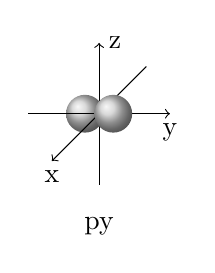
\begin{tikzpicture}[baseline=(current bounding box.center),scale=.6]
            \draw[->](0,-1.5)--(0,1.5)node[right]{z};
            \node[below] at (0,-2) {py};
            \shade[ball color=black!20] (-0.3,0)circle (0.4);
            \draw[->](-1.5,0)--(1.5,0)node[below]{y};
            \draw[->](1,1)--(-1,-1)node[below]{x};
            \shade[ball color=black!20] (0.3,0)circle (0.4);
        \end{tikzpicture}
    \end{subcaptionbox}
    \hfill
    \begin{subcaptionbox}
        \centering
        \begin{tikzpicture}[baseline=(current bounding box.center),scale=.6]
            \draw[->](-1.5,0)--(1.5,0)node[below]{y};
            \shade[ball color=black!20] (0,-0.3)circle (0.4);
            \draw[->](1,1)--(-1,-1)node[below]{x};
            \draw[->](0,-1.5)--(0,1.5)node[right]{z};
            \node[below] at (0,-2) {pz};
            \draw[-](-.6,.6)--(1.8,.6);
            \shade[ball color=black!20] (0,0.3)circle (0.4);
            \draw[-](-.6,.6)--(-1.8,-.6);
            \draw[-](-1.8,-.6)--(.6,-.6);
            \draw[-](.6,-.6)--(1.8,.6);
            \draw[->](1.2,.4)--(2,.8)node[right]{节面};
        \end{tikzpicture}
    \end{subcaptionbox}
    
    \begin{subcaptionbox}
        \centering
        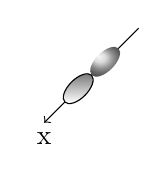
\begin{tikzpicture}[baseline=(current bounding box.center),scale=.6]
            \draw[->](1,1)--(-1,-1)node[below]{x};
            \begin{scope}[rotate around={45:(0.29,0.29)}]
                \shade[ball color=black!20] (0.29,0.29)ellipse (0.4 and 0.2);
            \end{scope}
            \begin{scope}[rotate around={45:(-0.28,-0.28)}]
                \shade[draw=black] (-0.28,-0.28)ellipse (0.4 and 0.2);
            \end{scope}
        \end{tikzpicture}
    \end{subcaptionbox}
    \hfill
    \begin{subcaptionbox}
        \centering
        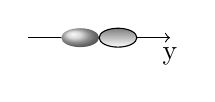
\begin{tikzpicture}[baseline=(current bounding box.center),scale=.6]
            \draw[->](-1.5,0)--(1.5,0)node[below]{y};
            \shade[ball color=black!20] (-0.4,0)ellipse (0.4 and 0.2);
            \shade[draw=black] (0.4,0)ellipse (0.4 and 0.2);
        \end{tikzpicture}
    \end{subcaptionbox}
    \hfill
    \begin{subcaptionbox}
        \centering
        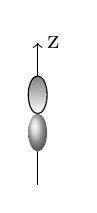
\begin{tikzpicture}[baseline=(current bounding box.center),scale=.6]
            \draw[->](0,-1.5)--(0,1.5)node[right]{z};
            \shade[ball color=black!20] (0,-0.4)ellipse (0.2 and 0.4);
            \shade[draw=black] (0,0.4)ellipse (0.2 and 0.4);
        \end{tikzpicture}
    \end{subcaptionbox}
    \caption{p轨道的几何分布}
    \label{f1.2}
\end{figure}

\begin{figure}[H]
    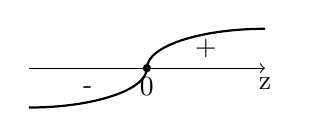
\begin{tikzpicture}
        \draw[->](-1.5,0)--(1.5,0)node[below]{z};
        \draw[ thick] (0,0) arc (0:-90:1.5 and 0.5);
        \draw[ thick, rotate=180] (0,0) arc (0:90:1.5 and -0.5);
        \draw[-](-0.75,-0.25)--(-0.75,-0.25)node[black]{-};
        \draw[-](0.75,0.25)--(0.75,0.25)node[black]{+};
        \fill [black] (0,0) circle (1.5pt) node[below] {0};
    \end{tikzpicture}
    相位:概率密度$\Psi^2=\Psi^*\Psi\left\{\begin{matrix} 
        \Psi<0\Rightarrow\Psi^2>0 \\
        \Psi>0\Rightarrow\Psi^2>0 \\
        \Psi=0\Rightarrow\Psi^2=0
     \end{matrix}\right.$
     
    $\underset{\text{节点/节面}}{\text{\uwave{相位为0}}}\begin{cases}
    \Psi_1=0 \\
    \Psi+\Psi_2=0(\Psi_1>0,\Psi_2<0)
     \end{cases}
     \begin{matrix}
        \Psi^2>0\quad \text{电子有分布} \\
        \Psi=0\quad \text{电子不会出现}
     \end{matrix}$
\end{figure}

\subsubsection{1.2.1.2轨道的能量}

单原子$:E_{1s}<E_{2s}<E_{2p}<E_{3s}<E_{3d}\dots$

\begin{figure}[H]
    \centering
    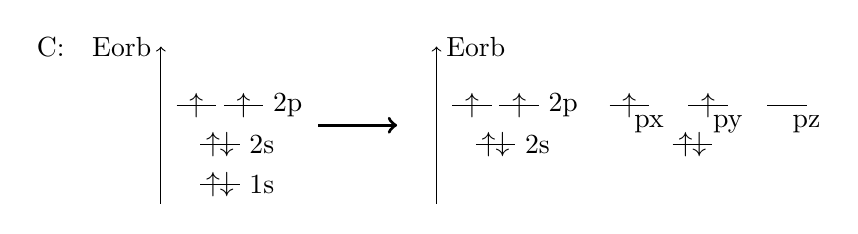
\begin{tikzpicture}[baseline=(current bounding box.center),scale=.5]
        \draw (1.6,2.5)--++(.5,0)node{$\uparrow$}-- ++(.5,0)node[right]{2p};
        \draw (0.4,2.5)--++(.5,0)node{$\uparrow$}-- ++(.5,0);
        \draw (1,1.5)--node{$\uparrow\downarrow$}+(1,0)node[right]{2s};
        \draw (1,0.5)--node{$\uparrow\downarrow$}+(1,0)node[right]{1s};
        \draw[->](0,0)--(0,4)node[left]{C:\quad Eorb};
        \draw[very thick, ->](4,2)--(6,2);
        \draw[->](7,0)--(7,4)node[right]{Eorb};
        \draw (8.6,2.5)--++(.5,0)node{$\uparrow$}-- ++(.5,0)node[right]{2p};
        \draw (7.4,2.5)--++(.5,0)node{$\uparrow$}-- ++(.5,0);
        \draw (8,1.5)--node{$\uparrow\downarrow$}+(1,0)node[right]{2s};
        \draw (15.4,2.5)--++(1,0)node[below]{pz};
        \draw (13.4,2.5)--++(.5,0)node{$\uparrow$}-- ++(.5,0)node[below]{py};
        \draw (11.4,2.5)--++(.5,0)node{$\uparrow$}-- ++(.5,0)node[below]{px};
        \draw (13,1.5)--node{$\uparrow\downarrow$}+(1,0);
    \end{tikzpicture}
\end{figure}

\subsection{价层电子互斥理论}
\label{sec:1.2.2}
\textcolor{red}{互斥:用定性的手段去解释空间结构}

\textcolor{red}{斥:远离配基(基团)$\rightarrow$满足斥力协调}

$\begin{cases}
    \text{中心原子(相对)} \\  
    \text{配基}\underset{\textcolor{red}{(\text{孤对电子})}}{\text{(基团)}}
 \end{cases}$
 斥力因素:$F_{\text{孤对-孤对}}>F_{\text{孤对-成键}}>F_{\text{成键-成键}}$

\begin{figure}[H]
    \centering
    \begin{subcaptionbox}
        \centering
        \begin{tikzpicture}[baseline=(current bounding box.center),scale=.6]
            \draw[draw=black] (1.3,1)ellipse (0.3 and 0.6);
            \chemfig{N(-[:-90,1.2]H)(-[:180,1.2]H)(-[:0,1.2]H)};
            \draw[->](3,0)--(5.5,0)node[above,pos=0.5]{不考虑}node[below,pos=0.5]{斥力大小};
            \fill (1.4,0.6) circle (1pt);
            \fill (1.2,0.6) circle (1pt);
        \end{tikzpicture}
    \end{subcaptionbox}
    \begin{subcaptionbox}
        \centering
        \begin{tikzpicture}[baseline=(current bounding box.center),scale=.6]
            \draw[draw=black] (0.9,1)ellipse (0.3 and 0.6);
            \chemfig{N(-[:-80,1.2]H)(-[:-30,1.2]H)(-[:-130,1.2]H)};
            \draw[->](3.5,0.2)--(5.5,0.2);
            \fill (1,0.6) circle (1pt);
            \fill (0.8,0.6) circle (1pt);
            \draw[<->] (1.5,-0.2) arc (0:25:3)node[right,pos=0.5]{$\underset{\text{实际107°}}{\text{109°}}$};
        \end{tikzpicture}
    \end{subcaptionbox}
    \begin{subcaptionbox}
        \centering
        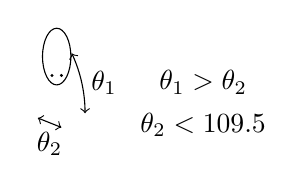
\begin{tikzpicture}[baseline=(current bounding box.center),scale=.6]
            \draw[draw=black] (0.9,1)ellipse (0.3 and 0.6);
            \chemfig{N(-[:-80,1.2]H)(-[:-30,1.2]H)(-[:-130,1.2]H)};
            \fill (1,0.6) circle (1pt);
            \fill (0.8,0.6) circle (1pt);
            \draw[<->] (1.5,-0.2) arc (0:25:3)node[right,pos=0.5]{$\theta_1$};
            \draw[<->] (1,-0.5)--(0.5,-0.3)node[below,pos=0.5]{$\theta_2$};
            \draw[-] (4,0)--(4,0)node[above,pos=0.5]{$\theta_1>\theta_2$}node[below,pos=0.5]{$\theta_2<109.5°$};
        \end{tikzpicture}
    \end{subcaptionbox}
\end{figure}

\subsection{定量地描绘空间结构}
\label{sec:1.2.3}
$\begin{cases} 
    \text{定量地描绘空间结构} \\  
    \text{巧妙运用“轨道”概念}
\end{cases}
\Rightarrow\underline{\text{杂化}}\text{轨道}
\begin{cases} 
    \text{杂}\textcolor{red}{\rightarrow\text{运用几种品类(s.p)}} \\  
    \text{化}\textcolor{red}{\rightarrow\text{重新组合s.p$\rightarrow$2条轨道}}
\end{cases}$

$\begin{cases} 
    \text{判断杂化方式}(\underset{\text{有机}}{\uwave{sp,sp^2,sp^3}},
    \underset{\text{无机}}{\uwave{\textcolor{red}{sp^2d,sp^3d,sp^3d^2,sp^3d^3}}}) \\
    \qquad\qquad\downarrow \\ 
    \text{轨道的几何关系} 
\end{cases}$

价层电子对数=$\frac{1}{2}(\text{中心原子主族序数+}\overset{\textcolor{red}{\sigma-1}}{\overset{\textcolor{red}{\pi-1}}{\text{配体数}}}+
\overset{\textcolor{red}{^{\ominus}+1}}{\overset{\textcolor{red}{^{\oplus}-1}}{\text{阴正阳负}}})$

$m\begin{cases}
    m=4,sp^3 \\
    m=3,sp^2 \\
    m=2,sp
\end{cases}
\qquad\qquad
\begin{matrix}
    ^{\oplus}CH_3=\frac{1}{2}(4+3-1)=3\Rightarrow{sp^2} \\
    ^{\ominus}CH_3=\frac{1}{2}(4+3+1)=4\Rightarrow{sp^3}
\end{matrix}$

\begin{figure}[H]
    \centering
    \begin{subcaptionbox}
        \centering
        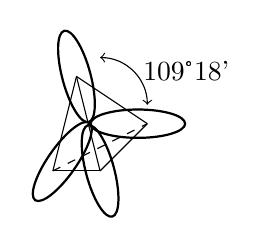
\begin{tikzpicture}[baseline=(current bounding box.center),scale=.6]
            \draw[-](0.5,-1)--(-0.5,-1);
            \draw[-](-0.5,-1)--(0,1);
            \draw[-](0,1)--(0.5,-1);
            \draw[-](0,1)--(1.5,0);
            \draw[-](0.5,-1)--(1.5,0);
            \draw[-,dashed](-0.5,-1)--(1.5,0);
            \begin{scope}[rotate around={105:(0.5,-1)}]
                \draw[thick] (0.5,-1) ellipse (1 and 0.3);
            \end{scope}
            \begin{scope}[rotate around={55:(-0.3,-0.8)}]
                \draw[thick] (-0.3,-0.8) ellipse (1 and 0.3);
            \end{scope}
            \begin{scope}[rotate around={105:(0,1)}]
                \draw[thick] (0,1) ellipse (1 and 0.3);
            \end{scope}
            \begin{scope}[rotate around={0:(1.3,0)}]
                \draw[thick] (1.3,0) ellipse (1 and 0.3);
            \end{scope}
            \draw[<->] (1.5,0.4) arc (0:90:1)node[right,pos=0.5]{109°18'};
        \end{tikzpicture}
    \end{subcaptionbox}
    \hfill
    \begin{subcaptionbox}
        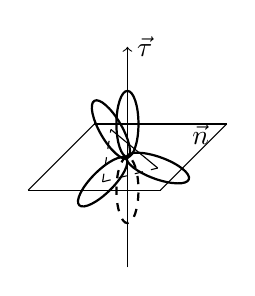
\begin{tikzpicture}[baseline=(current bounding box.center),scale=.7]
            \draw[->](0,-2)--(0,2)node[right]{$\vec{\tau}$};
            \draw[-](-.6,.6)--(1.8,.6);
            \draw[-](-.6,.6)--(-1.8,-.6);
            \draw[-](-1.8,-.6)--(.6,-.6);
            \draw[-](.6,-.6)--(1.8,.6);
            \node[right] at (1,.4){$\vec{n}$};
            \begin{scope}[rotate around={90:(0,0.6)}]
                \draw[thick] (0,0.6) ellipse (0.6 and 0.2);
            \end{scope}
            \begin{scope}[rotate around={90:(0,-0.6)}]
                \draw[thick,dashed] (0,-0.6) ellipse (0.6 and 0.2);
            \end{scope}
            \begin{scope}[rotate around={45:(-0.45,-0.45)}]
                \draw[thick] (-0.45,-0.45) ellipse (0.6 and 0.2);
            \end{scope}
            \begin{scope}[rotate around={160:(0.55,-0.2)}]
                \draw[thick] (0.55,-0.2) ellipse (0.6 and 0.2);
            \end{scope}
            \begin{scope}[rotate around={120:(-0.3,0.5)}]
                \draw[thick] (-0.3,0.5) ellipse (0.6 and 0.2);
            \end{scope}
            \draw[-,dashed](-0.45,-0.45)--(0.55,-0.2);
            \draw[-,dashed](-0.45,-0.45)--(-0.3,0.5);
            \draw[-](0.55,-0.2)--(-0.3,0.5);
        \end{tikzpicture}
    \end{subcaptionbox}
    \hfill
    \begin{subcaptionbox}
        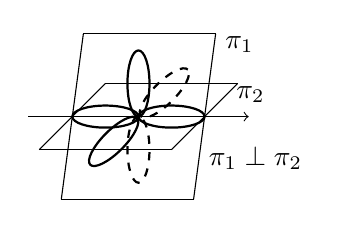
\begin{tikzpicture}[baseline=(current bounding box.center),scale=.7]
            \draw[->](-2,0)--(2,0);
            \draw[-](-.6,.6)--(1.8,.6);
            \draw[-](-.6,.6)--(-1.8,-.6);
            \draw[-](-1.8,-.6)--(.6,-.6);
            \draw[-](.6,-.6)--(1.8,.6);
            \node[right] at (1.6,.4){$\pi_2$};
            \begin{scope}[rotate around={90:(0,0.6)}]
                \draw[thick] (0,0.6) ellipse (0.6 and 0.2);
            \end{scope}
            \begin{scope}[rotate around={90:(0,-0.6)}]
                \draw[thick,dashed] (0,-0.6) ellipse (0.6 and 0.2);
            \end{scope}
            \begin{scope}[rotate around={0:(0.6,0)}]
                \draw[thick] (0.6,0) ellipse (0.6 and 0.2);
            \end{scope}
            \begin{scope}[rotate around={0:(-0.6,0)}]
                \draw[thick] (-0.6,0) ellipse (0.6 and 0.2);
            \end{scope}
            \begin{scope}[rotate around={45:(-0.45,-0.45)}]
                \draw[thick] (-0.45,-0.45) ellipse (0.6 and 0.2);
            \end{scope}
            \begin{scope}[rotate around={45:(0.4,0.5)}]
                \draw[thick,dashed] (0.4,0.4) ellipse (0.6 and 0.2);
            \end{scope}
            \draw[-](-1,1.5)--(1.4,1.5);
            \draw[-](-1,1.5)--(-1.4,-1.5);
            \draw[-](1,-1.5)--(1.4,1.5)node[right,pos=0.25]{$\pi_1\perp\pi_2$};
            \draw[-](-1.4,-1.5)--(1,-1.5);
            \node[right] at (1.4,1.3){$\pi_1$};
        \end{tikzpicture}
    \end{subcaptionbox}
\end{figure}

$\underset{\text{孤对电子数}}{AX_n:}^nLp=\overset{\textcolor{red}{\text{价层电子对数}}}{\overset{\textcolor{red}{\uparrow}}{m}}-
\underset{\textcolor{red}{\text{配体}}}{\underset{\textcolor{red}{\downarrow}}{n}}$

\begin{figure}[H]
    \begin{tikzpicture}[baseline=(current bounding box.center),scale=.5]
        \draw (2.8,2.5)--++(1,0)node[right]{2p};
        \draw (1.6,2.5)--++(.5,0)node{$\uparrow$}-- ++(.5,0);
        \draw (0.4,2.5)--++(.5,0)node{$\uparrow$}-- ++(.5,0);
        \draw (1,1.5)--node{$\uparrow\downarrow$}+(1,0)node[right]{2s};
        \draw[->](0,0)--(0,4)node[right]{Eorb}node[left]{杂化之前};
    \end{tikzpicture}
\end{figure}


\begin{figure}[H]
    \qquad
    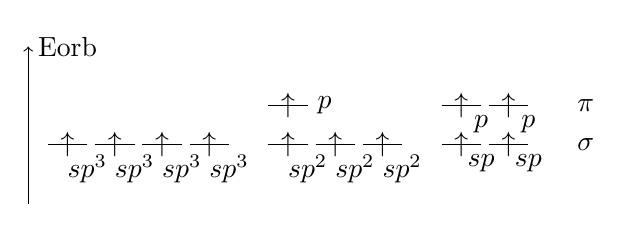
\begin{tikzpicture}[baseline=(current bounding box.center),scale=.5]
        \draw[->](0,0)--(0,4)node[right]{Eorb};
        \draw (0.5,1.5)--++(.5,0)node{$\uparrow$}-- ++(.5,0)node[below]{$sp^3$};
        \draw (1.7,1.5)--++(.5,0)node{$\uparrow$}-- ++(.5,0)node[below]{$sp^3$};
        \draw (2.9,1.5)--++(.5,0)node{$\uparrow$}-- ++(.5,0)node[below]{$sp^3$};
        \draw (4.1,1.5)--++(.5,0)node{$\uparrow$}-- ++(.5,0)node[below]{$sp^3$};
        \draw (6.1,1.5)--++(.5,0)node{$\uparrow$}-- ++(.5,0)node[below]{$sp^2$};
        \draw (7.3,1.5)--++(.5,0)node{$\uparrow$}-- ++(.5,0)node[below]{$sp^2$};
        \draw (8.5,1.5)--++(.5,0)node{$\uparrow$}-- ++(.5,0)node[below]{$sp^2$};
        \draw (6.1,2.5)--++(.5,0)node{$\uparrow$}-- ++(.5,0)node[right]{$p$};
        \draw (10.5,1.5)--++(.5,0)node{$\uparrow$}-- ++(.5,0)node[below]{$sp$};
        \draw (11.7,1.5)--++(.5,0)node{$\uparrow$}-- ++(.5,0)node[below]{$sp$};
        \draw (10.5,2.5)--++(.5,0)node{$\uparrow$}-- ++(.5,0)node[below]{$p$};
        \draw (11.7,2.5)--++(.5,0)node{$\uparrow$}-- ++(.5,0)node[below]{$p$};
        \node[right] at (13.7,1.5){$\sigma$};
        \node[right] at (13.7,2.5){$\pi$};
    \end{tikzpicture}
\end{figure}

按实际成键方式填电子

\section{价键理论,分子轨道理论}
\label{sec:1.3}
杂化轨道理论只解决了中心原子的杂化问题,化学键的本质仍然没有说明

提论
$\begin{cases}
    VBT\quad \text{价键理论}\Rightarrow\textcolor{red}{\text{“交换电子”$\rightleftarrows\text{共振}\rightarrow\text{共振论}\leftarrow$Lewis结构式}} \\
    MOT\quad \text{分子轨道理论}
\end{cases}$

在有机中,往往把VBT与MOT结合起来,并侧重于MOT的应用

$\textcolor{red}{\uwave{\textcolor{black}{\text{原子之间通过共享电子}}}}
\overset{\textcolor{red}{\text{共价键}}}{\overset{\textcolor{red}{\uparrow}}{\textcolor{red}{\uwave{\textcolor{black}{\text{成键}}}}}}
\rightarrow\text{为什么倾向成键}\textcolor{red}{\ce{->[\text{本质}]}\text{成键后能量降低}}$

\begin{figure}[H]
    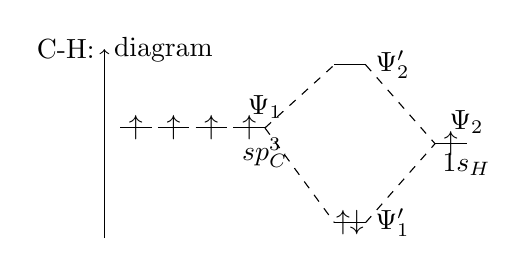
\begin{tikzpicture}[baseline=(current bounding box.center),scale=.4]
        \draw[->](0,-2)--(0,4)node[right]{diagram}node[left]{C-H:};
        \draw (0.5,1.5)--++(.5,0)node{$\uparrow$}-- ++(.5,0);
        \draw (1.7,1.5)--++(.5,0)node{$\uparrow$}-- ++(.5,0);
        \draw (2.9,1.5)--++(.5,0)node{$\uparrow$}-- ++(.5,0);
        \draw (4.1,1.5)--++(.5,0)node{$\uparrow$}-- ++(.5,0)node[below]{$sp_C^3$}node[above]{$\Psi_1$};
        \draw[-,dashed](5.1,1.5)--(7.3,3.5);
        \draw[-,dashed](5.1,1.5)--(7.3,-1.5);
        \draw (7.3,3.5)--++(1,0)node[right]{$\Psi_2'$};
        \draw (7.3,-1.5)--node{$\uparrow\downarrow$}+(1,0)node[right]{$\Psi_1'$};
        \draw[-,dashed](8.3,3.5)--(10.5,1);
        \draw[-,dashed](8.3,-1.5)--(10.5,1);
        \draw (10.5,1)--++(.5,0)node{$\uparrow$}-- ++(.5,0)node[below]{$1s_H$}node[above]{$\Psi_2$};
    \end{tikzpicture}
    $\left.\begin{matrix}
        C\text{的}sp_C^3 \\
        H\text{的}1s_H
    \end{matrix}\right\}\text{重新组合}\left\{\begin{matrix}
        \Psi_1' \\
        \Psi_2'
    \end{matrix}\right.\text{新的轨道}$

    \text{由于组合生成的轨道已经包含于分子中\quad $\therefore$叫“分子轨道”}
\end{figure}

$E_{\Psi_2'}>E_{\Psi_1'}
\begin{cases}
    e^-\text{在$\Psi_1$中,能量有降低倾向}\textcolor{red}{\rightarrow\text{CH共享电子}\rightarrow\text{形成C-H键}} \\
    e^-\text{在$\Psi_2$中,能量有升高倾向}\textcolor{red}{\rightarrow\text{瓦解C-H键}}
\end{cases}$

$\Psi_1:\sigma_{C-H}(\text{C-H成键}\sigma\text{轨道})$

$\Psi_2:\sigma^*_{C-H}(\text{C-H反键}\sigma\text{轨道})$

如何重新组合$\Rightarrow$原波函数线性组合(LCAO)

推论:若$e^-\text{填到了}\sigma$上,有形成化学键的倾向(成键本质)

若$e^-\text{填到了}\sigma^*$上,有瓦解化学键的倾向(断键本质)

\begin{figure}[H]
    $\begin{cases}
    \Psi_2+\Psi_1=\Psi_1' \\
    \Psi_2-\Psi_1=\Psi_2'
    \end{cases}$
    \begin{tikzpicture}[baseline=(current bounding box.center),scale=.5]
        \draw[draw=black] (-0.4,0)ellipse (0.4 and 0.2);
        \shade[ball color=black!20] (0.6,0)ellipse (0.6 and 0.3);
        \draw[draw=black] (-0.4,1)ellipse (0.4 and 0.2);
        \shade[ball color=black!20] (0.6,1)ellipse (0.6 and 0.3);
        \node[right] at (1.5,1) {$+$};
        \node[right] at (1.5,0) {$+$};
        \shade[ball color=black!20] (3,1)circle (0.3);
        \draw[draw=black] (3,0)circle (0.3);
        \draw[->] (3.5,1)--(4,1)node[right]{$\sigma$};
        \draw[->] (3.5,0)--(4,0)node[right]{$\sigma^*$};
        \draw[-,red] (5,-0.4)--(15.5,-0.4)node[right]{};
        \draw[-,red] (5,1.4)--(15.5,1.4)node[red,right]{$\star$};
        \draw[-,red] (5,-0.4)--(5,1.4)node[red,right,pos=0.5]{轨道有效重叠的程度越高,整体能量越低};
        \draw[-,red] (15.5,-0.4)--(15.5,1.4)node[right]{};
    \end{tikzpicture}
\end{figure}

$\left.\begin{matrix}
    \textcolor{red}{\text{正相位+正相位}} \\
    \textcolor{red}{\text{程度最大}}
\end{matrix}\right\}\textcolor{red}{\text{有效重叠}}\rightarrow\text{解释为什么在“轴向”$\sigma$键}$

关于分子轨道理论的几大概念

\qquad 注:一个分子有几条化学键$\Rightarrow$几组分子轨道

\qquad 我们一般分析“某条化学键”的分子轨道

\subsection{充满轨道与空轨道}
\label{sec:1.3.1}
\begin{figure}[H]
    \begin{tikzpicture}[baseline=(current bounding box.center),scale=.5]
        \draw (1,4)--++(1,0)node[right]{$\Psi_4$};
        \draw (1,3)--++(1,0)node[right]{$\Psi_3$};
        \draw (1,2)--node{$\uparrow\downarrow$}+(1,0)node[right]{$\Psi_2$};
        \draw (1,1)--node{$\uparrow\downarrow$}+(1,0)node[right]{$\Psi_1$};
        \draw[->](0,0)--(0,4.5)node[left]{Eorb};
        \node[above] at (6,3) {$\Psi_1\Psi_2$为充满轨道};
        \node[below] at (6,3) {$\Psi_3\Psi_4$为充满轨道};
        \draw[->,red] (4.5,2)--(5,1)node[red,right]{基态:$E_{\text{充满}}<E_{\text{空}}$};
    \end{tikzpicture}
\end{figure}

\subsection{孤对电子的分子轨道}
\label{sec:1.3.2}
\begin{figure}[H]
    \text{孤对电子的分子轨道$\rightarrow$孤对电子不参与成键,可以叫做“非键”}
    
    \begin{tikzpicture}[baseline=(current bounding box.center),scale=.4]
        \draw[->](0,-2)--(0,4)node[right]{以$CH_3$为例:};
        \draw (0.5,1.5)--node{$\uparrow\downarrow$}+(1,0)node[below]{$sp^3$};
        \draw (1.7,1.5)--++(.5,0)node{$\uparrow$}-- ++(.5,0)node[below]{$sp^3$};
        \draw (2.9,1.5)--++(.5,0)node{$\uparrow$}-- ++(.5,0)node[below]{$sp^3$};
        \draw (4.1,1.5)--++(.5,0)node{$\uparrow$}-- ++(.5,0)node[below]{$sp^3$};
        \draw[-](1.7,0.5)--(5.1,0.5)node[pos=0.5,below]{与3个H的1s成键};
        \draw[-,dashed](5.1,1.5)--(6.3,3.5);
        \draw[-,dashed](5.1,1.5)--(6.3,-1.5);
        \draw (6.3,3.5)--++(1,0)node[right]{$\sigma^*_{N-H}$};
        \draw (6.3,-1.5)--node{$\uparrow\downarrow$}+(1,0)node[right]{$\sigma_{N-H}$};
        \draw[-,dashed](7.3,3.5)--(8.5,1);
        \draw[-,dashed](7.3,-1.5)--(8.5,1);
        \draw (8.5,1)--++(.5,0)node{$\uparrow$}-- ++(.5,0)node[below]{$1s_H$};
        \draw[->](10.5,1.5)--(14,1.5)node[red,pos=0.5,above]{简化}node[red,pos=0.5,below]{省略组合过程};
        \draw[->](15.5,-2)--(15.5,4)node[right]{Eorb};
        \draw (16,0)--node{$\uparrow\downarrow$}+(1,0);
        \draw (17.2,0)--node{$\uparrow\downarrow$}+(1,0);
        \draw (18.4,0)--node{$\uparrow\downarrow$}+(1,0)node[right]{3个$\sigma_{N-H}$};
        \draw (17.2,1.5)--node{$\uparrow\downarrow$}+(1,0)node[right]{$sp_N^3$};
        \draw[->](20,1.5)--(21,1.5)node[right]{孤对电子保持原有轨道};
        \draw (16,3)--++(1,0);
        \draw (17.2,3)--++(1,0);
        \draw (18.4,3)--++(1,0)node[right]{3个$\sigma^*_{N-H}$};
    \end{tikzpicture}
\end{figure}

\subsection{$\sigma\text{轨道与}\pi$轨道}
\label{sec:1.3.3}
$\sigma\text{轨道与}\pi\text{轨道}$
$\begin{cases}
    \text{成$\sigma$键}
    \begin{cases}
        \sigma^*_{A-B} \\
        \sigma_{A-B}
    \end{cases} \\
    \text{成$\pi$键}
    \begin{cases}
        \pi^*_{A-B} \\
        \pi_{A-B}
    \end{cases}
\end{cases}
\text{能量关系:}E^*_{\sigma}>E^*_{\pi}>\overset{\textcolor{red}{\text{非键}}}{\overset{\textcolor{red}{\uparrow}}{E_n}}>E_{\pi}>E_{\sigma}$

\begin{figure}[H]
    \begin{tikzpicture}[baseline=(current bounding box.center),scale=.5]
        \draw[->](0,-2)--(0,5)node[left]{双键的形成}node[right]{Erob};
        \draw (1,-0.25)--++(.5,0)node{$\uparrow$}-- ++(.5,0)node[left,pos=0]{$sp^2$};
        \draw[-,dashed](2,-0.25)--(4,5);
        \draw[-,dashed](2,-0.25)--(4,-1.5);
        \draw (1,2.25)--++(.5,0)node{$\uparrow$}-- ++(.5,0)node[left,pos=0]{$2p$};
        \draw[-,dashed](2,2.25)--(4,4);
        \draw[-,dashed](2,2.25)--(4,1);
        \draw (4,-1.5)--node{$\uparrow\downarrow$}+(1,0)node[right]{$\sigma$};
        \draw (4,1)--node{$\uparrow\downarrow$}+(1,0)node[right]{$\pi$};
        \draw (4,4)--++(1,0)node[right]{$\pi^*$};
        \draw (4,5)--++(1,0)node[right]{$\sigma^*$};
        \draw (7,0.25)--++(.5,0)node{$\uparrow$}-- ++(.5,0)node[right]{$sp^2$};
        \draw[-,dashed](7,0.25)--(5,5);
        \draw[-,dashed](7,0.25)--(5,-1.5);
        \draw (7,2.75)--++(.5,0)node{$\uparrow$}-- ++(.5,0)node[right]{$2p$};
        \draw[-,dashed](7,2.75)--(5,4);
        \draw[-,dashed](7,2.75)--(5,1);
        \draw[->](6,4)--(10,4.5);
        \shade[ball color=black!20] (11,4.9)ellipse (0.2 and 0.4);
        \draw[draw=black] (11,4.1)ellipse (0.2 and 0.4);
        \node[black] at (12.5,4.5) {+};
        \draw[draw=black] (14,4.9)ellipse (0.2 and 0.4);
        \shade[ball color=black!20] (14,4.1)ellipse (0.2 and 0.4);
        \draw[->](15,4.5)--(16,4.5);
        \begin{scope}[rotate around={45:(16.5,4.1)}]
            \draw[draw=black] (16.5,4.1)ellipse (0.4 and 0.2);
        \end{scope}
        \begin{scope}[rotate around={45:(17.5,4.9)}]
            \draw[draw=black] (17.5,4.9)ellipse (0.4 and 0.2);
        \end{scope}
        \begin{scope}[rotate around={135:(16.5,4.9)}]
            \shade[ball color=black!20] (16.5,4.9)ellipse (0.4 and 0.2);
        \end{scope}
        \begin{scope}[rotate around={135:(17.5,4.1)}]
            \shade[ball color=black!20] (17.5,4.1)ellipse (0.4 and 0.2);
        \end{scope}
        \node[black] at (18,4.5) {$\pi^*$};
        \draw[->](6,1)--(10,0.5);
        \shade[ball color=black!20] (11,0.9)ellipse (0.2 and 0.4);
        \draw[draw=black] (11,0.1)ellipse (0.2 and 0.4);
        \node[black] at (12.5,0.5) {+};
        \shade[ball color=black!20] (14,0.9)ellipse (0.2 and 0.4);
        \draw[draw=black] (14,0.1)ellipse (0.2 and 0.4);
        \draw[->](15,0.5)--(16,0.5);
        \shade[ball color=black!20] (17,0.8)ellipse (0.4 and 0.2);
        \draw[draw=black] (17,0.2)ellipse (0.4 and 0.2);
        \node[black] at (18,0.5) {$\pi$};
    \end{tikzpicture}
\end{figure}

\subsection{简单的轨道能量关系}
\label{sec:1.3.4}
\begin{figure}[H]
    \begin{tikzpicture}[baseline=(current bounding box.center),scale=.4]
        \draw (1,4)--++(1,0)node[right]{$\sigma^*$};
        \draw (1,3)--++(1,0)node[right]{$\pi^*$};
        \draw (1,2)--++(1,0)node[right]{$n$};
        \draw (1,1)--++(1,0)node[right]{$\pi$};
        \draw (1,0)--++(1,0)node[right]{$\sigma$};
        \draw[->](0,-1)--(0,5)node[right]{Eorb}node[left,pos=0.25]{断键\quad $\text{优先}\pi\text{,其次}\sigma$}node[left,pos=0.75]{给电子能力\quad 单键<双键<孤对电子};
    \end{tikzpicture}
    $\text{某些杂化轨道}\begin{cases}
        \text{空的p轨道} \\
        \text{孤对电子占据轨道}
    \end{cases}$
\end{figure}

该关系为之后介绍某些反应为什么能量能够发生提供理论基础

\begin{figure}[H]
    \centering
    \begin{tikzpicture}[baseline=(current bounding box.center),scale=.4]
        \draw[<-](0,0)--(0,5)node[above]{结构理论:}node[below,pos=0]{反应理论:};
        \node[above] at (5,5) {Lewis$e^-$配对};
        \node[below] at (5,5) {原子轨道};
        \node[above] at (5,3) {VSEPR};
        \node[below] at (5,3) {杂化轨道};
        \node[above] at (5,1) {VBT};
        \node[below] at (5,1) {MOT};
        \node[below] at (5,0) {电负性};
        \draw[->](5,-1)--(5,-2)node[right]{分子有极性(偶极模型)};
        \node[right] at (12,-3) {+碰撞理论$\rightarrow$机理};
    \end{tikzpicture}
\end{figure}

\qquad\qquad\qquad\qquad\qquad MOT

\qquad\qquad\qquad\qquad\qquad\quad $\downarrow$

\qquad\qquad\qquad\qquad\qquad HOMO/LUMO(前线轨道理论)